Once the HestiaPi Touch boots, the interface will have a simple interface to
adjust the heating, cooling, or fan.  It also displays the current temperature
and humidity, as well as an icon in the upper right to get technical
information about the Pi.  The interface immediately after boot is shown in
figure \ref{fig:ui}.

\begin{figure}
\centering
\begin{subfigure}{0.5\textwidth}
  \centering
  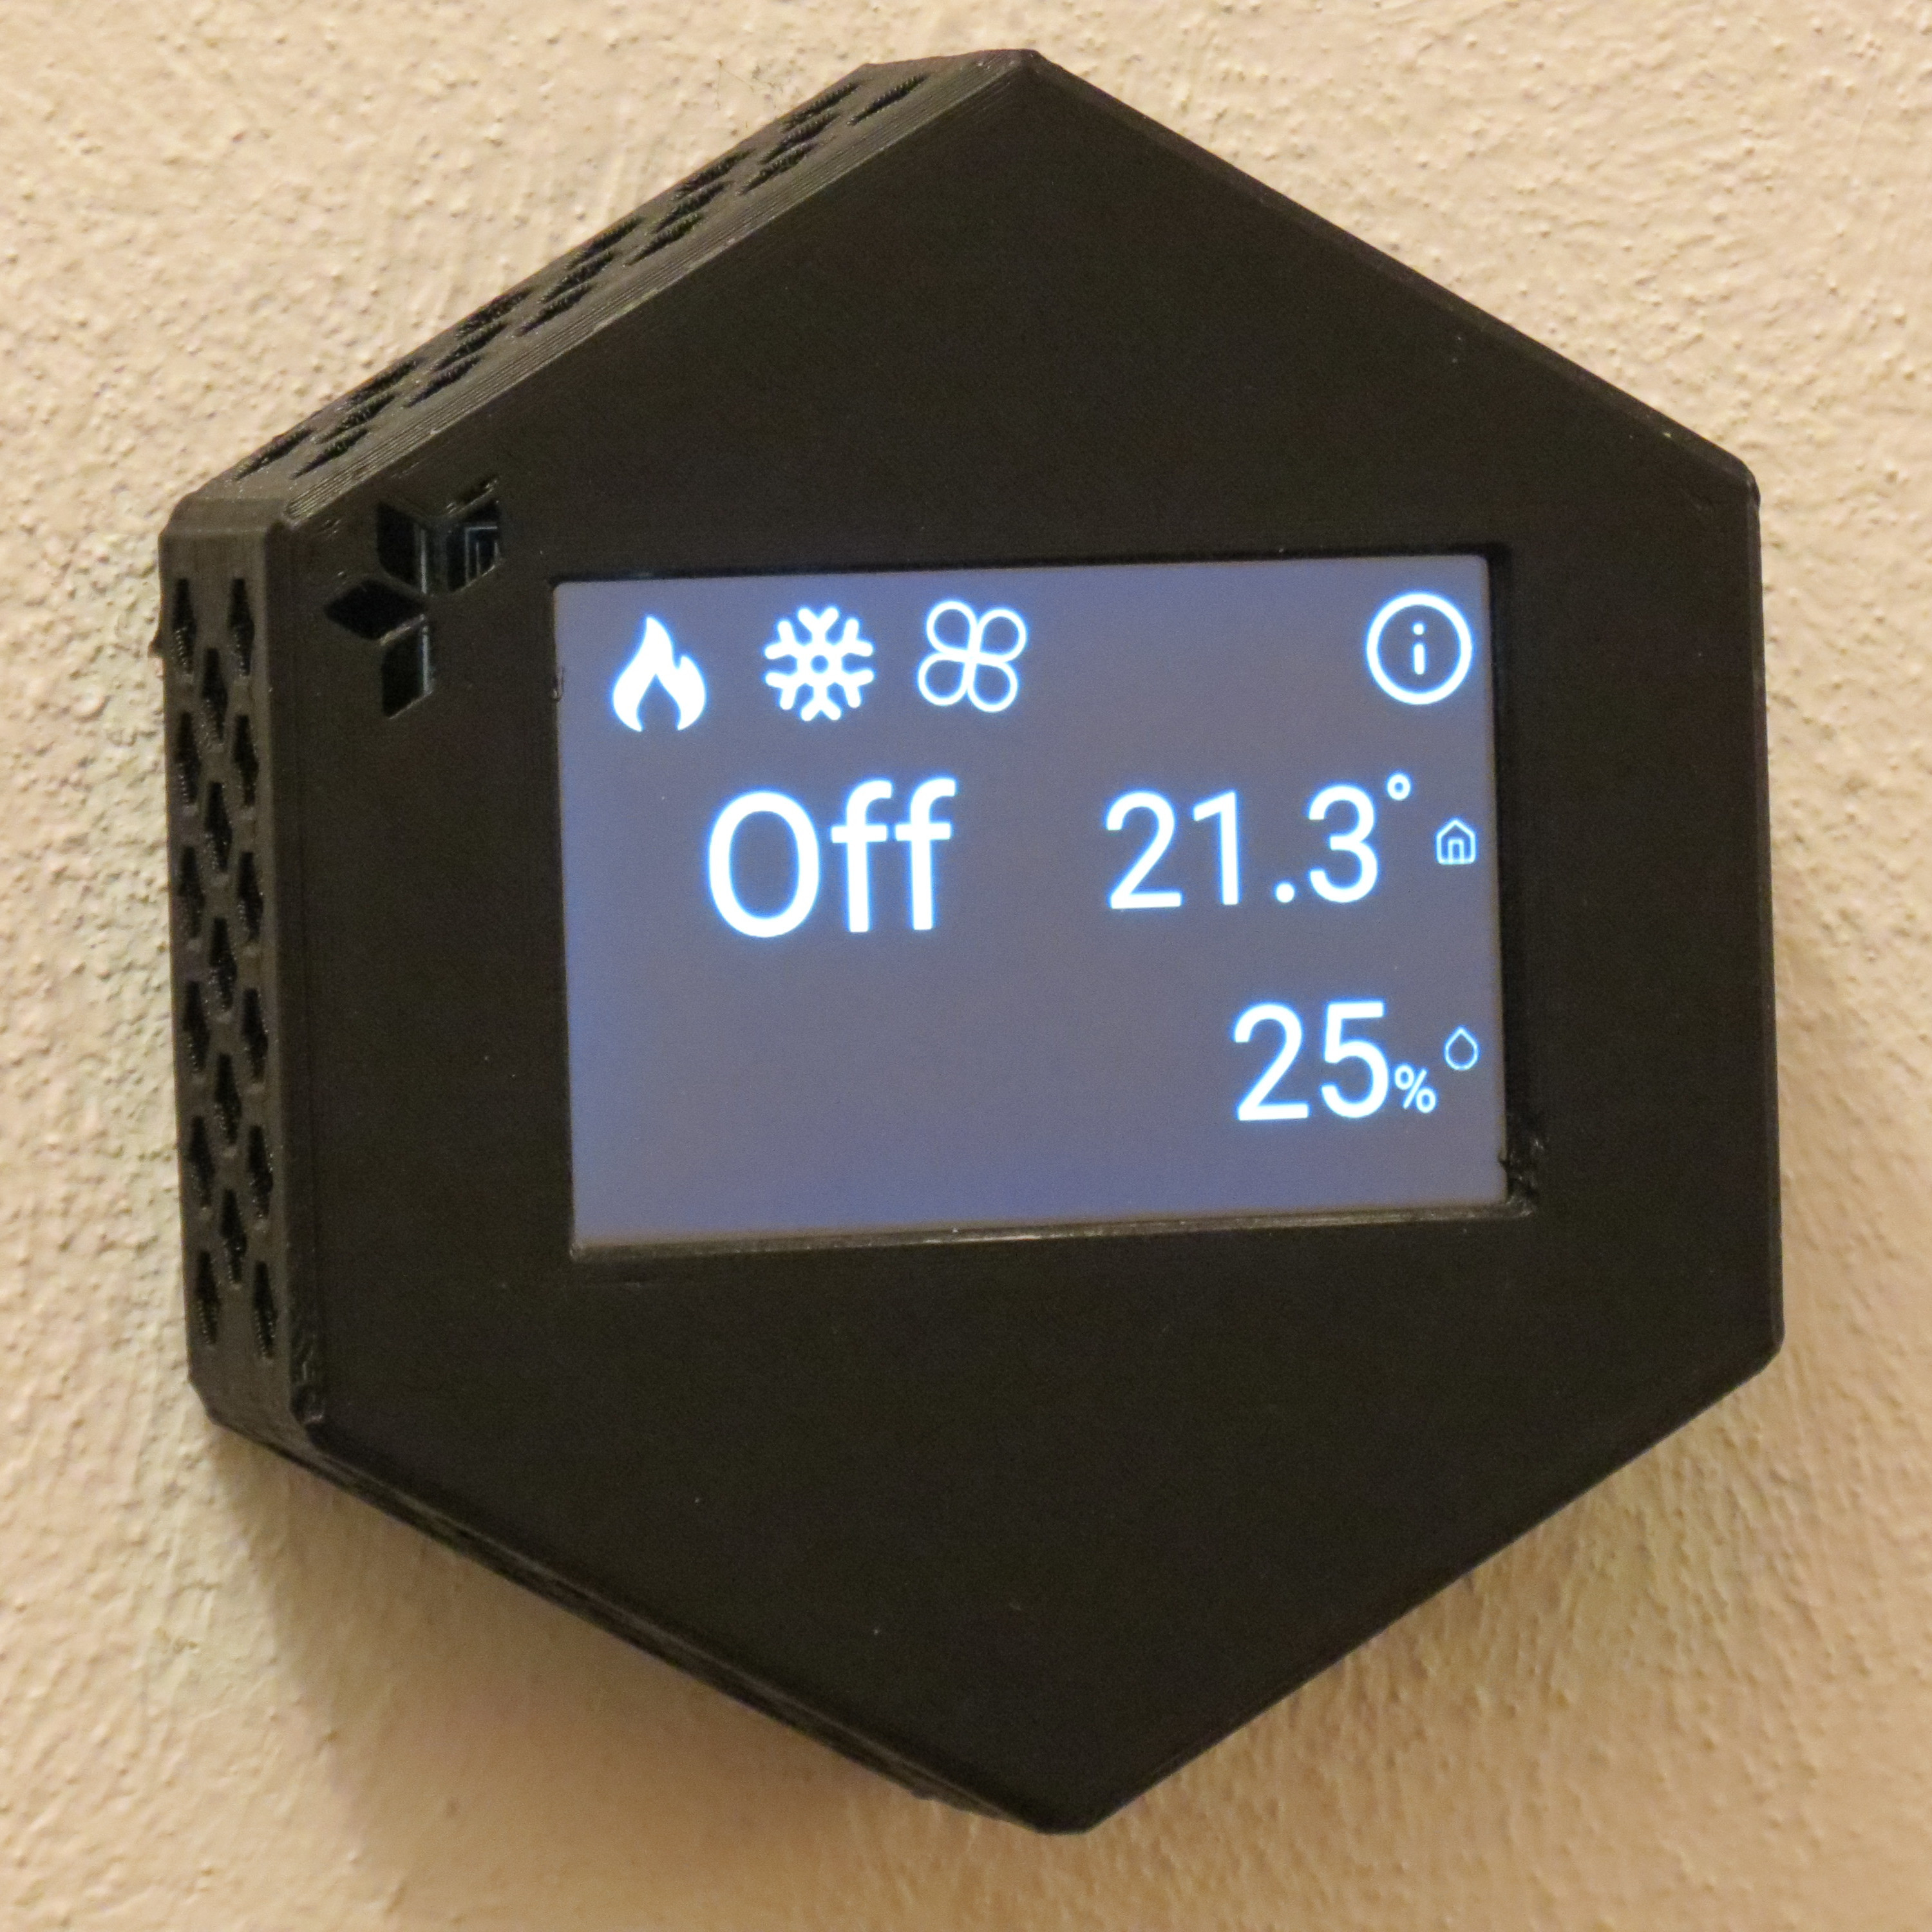
\includegraphics[width=.75\linewidth]{img/ui.jpg}
  \caption{User Interface After Booting}
  \label{fig:ui}
\end{subfigure}%
\begin{subfigure}{0.5\textwidth}
  \centering
  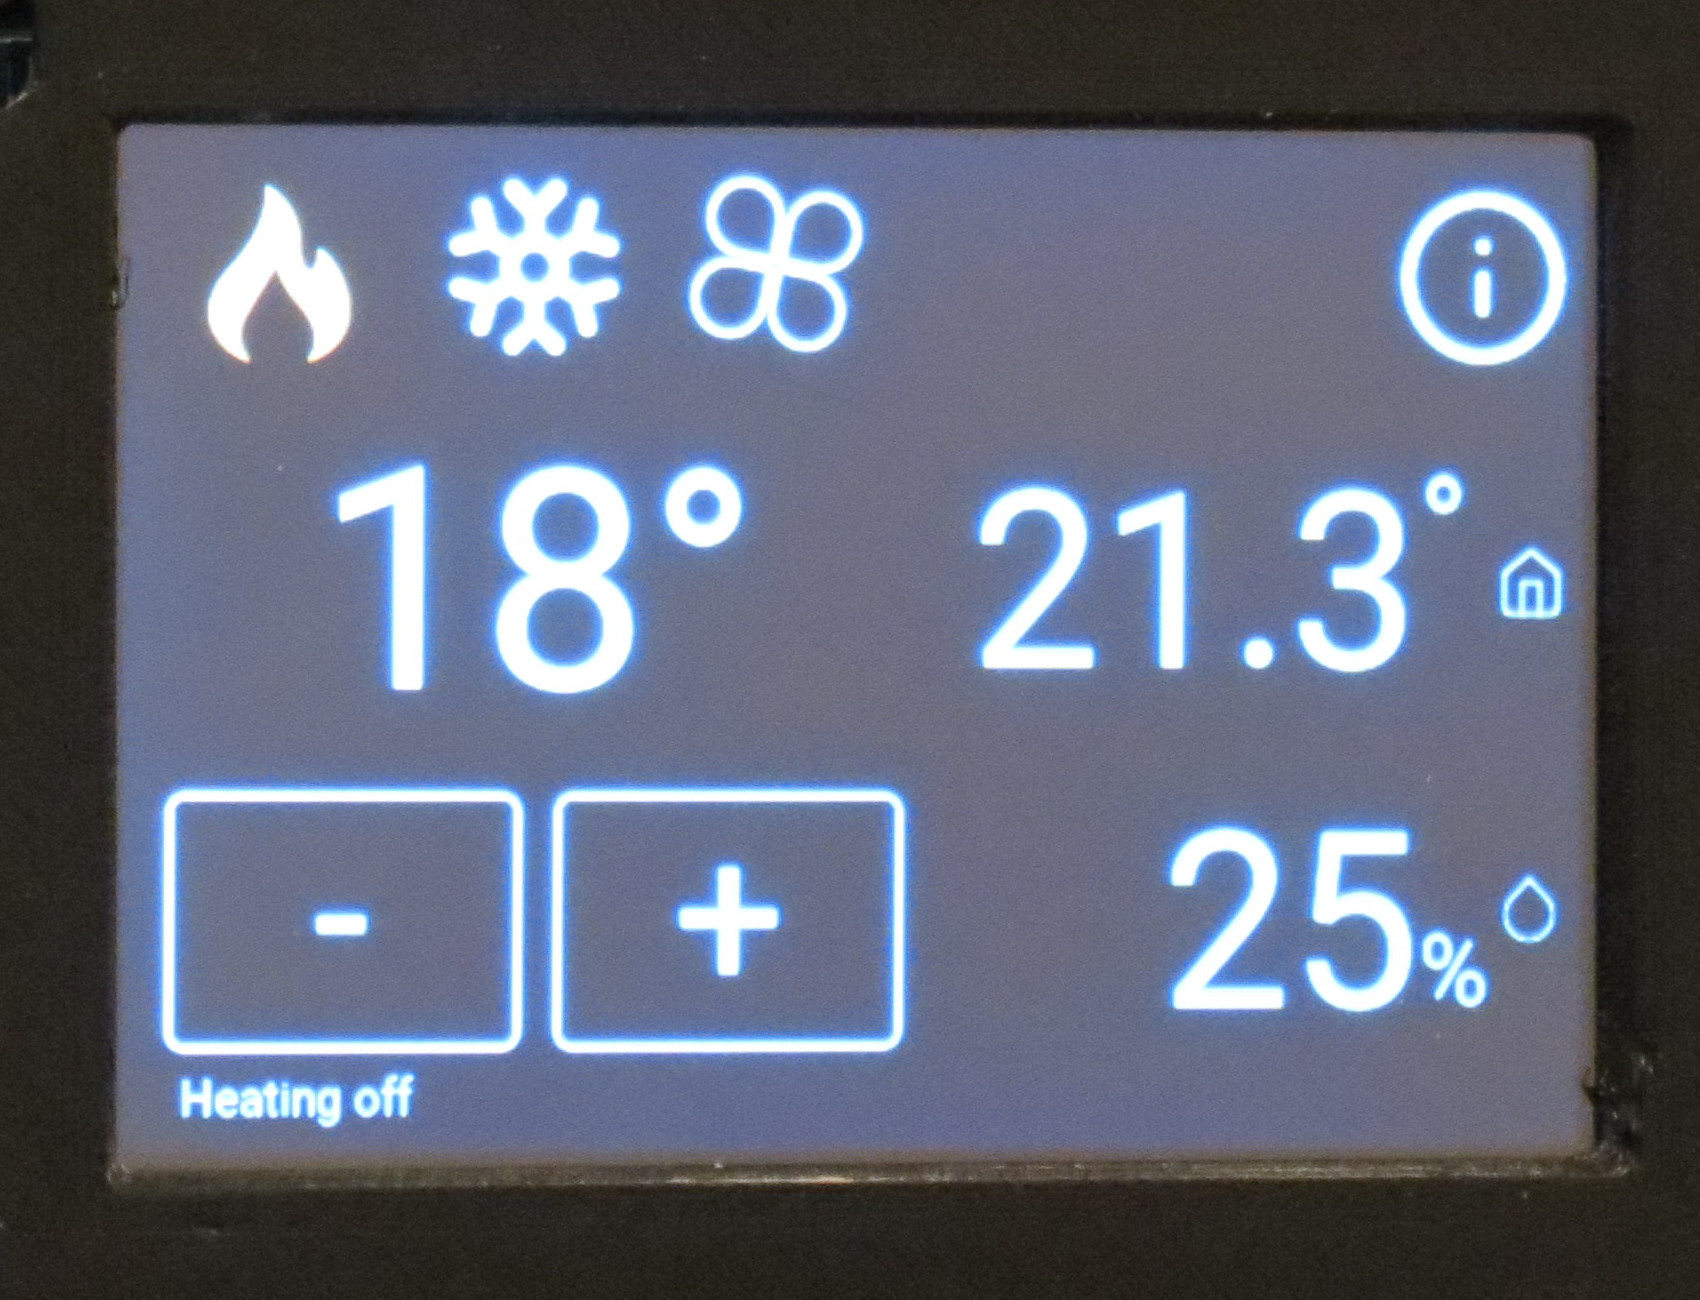
\includegraphics[width=.75\linewidth]{img/ui-heating-off.jpg}
  \caption{Heating Interface - Heat is off}
  \label{fig:ui-heating-off}
\end{subfigure}

\begin{subfigure}{0.5\textwidth}
  \centering
  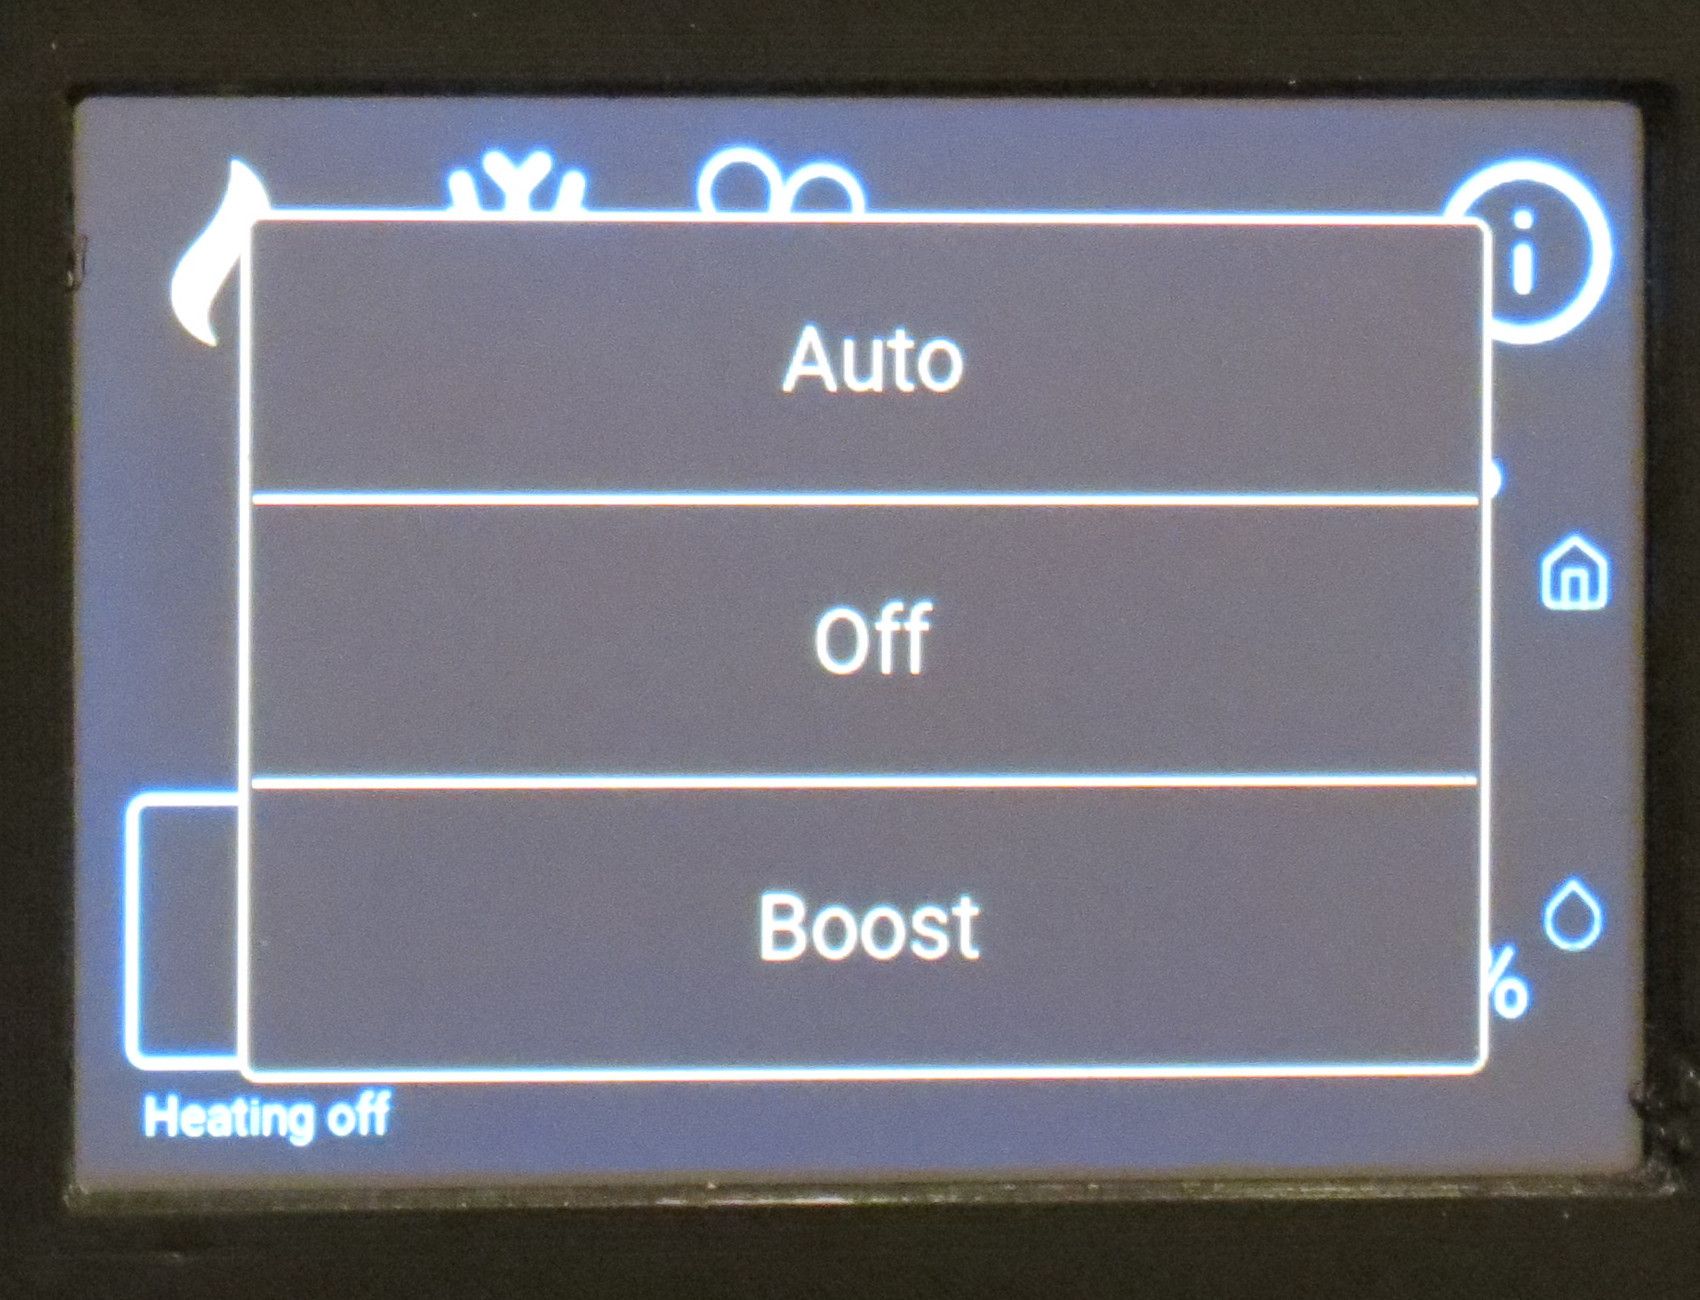
\includegraphics[width=.75\linewidth]{img/ui-heating-menu.jpg}
  \caption{Heating Interface - Toggle heat on/off}
  \label{fig:ui-heating-menu}
\end{subfigure}%
\begin{subfigure}{0.5\textwidth}
  \centering
  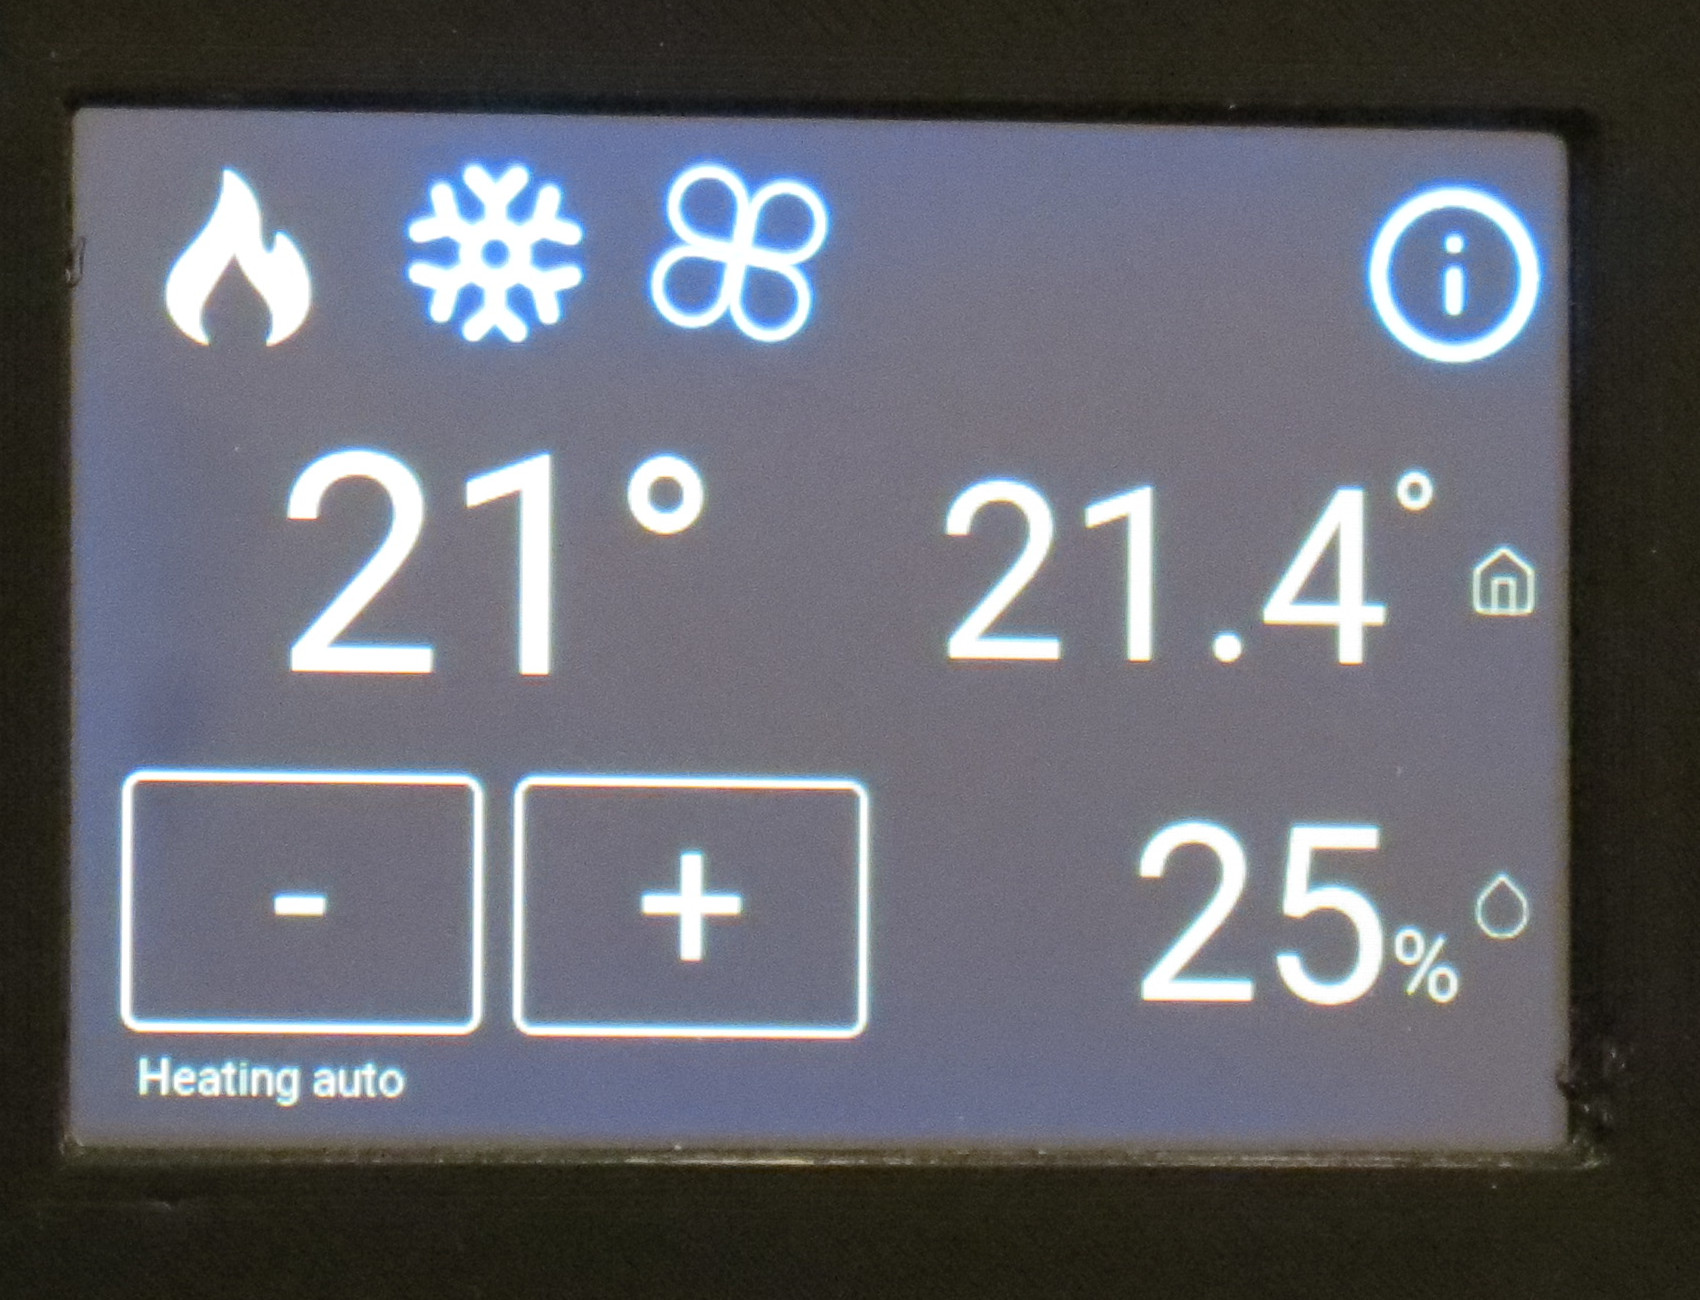
\includegraphics[width=.75\linewidth]{img/ui-heating-on.jpg}
  \caption{Heating Interface - The heat is on}
  \label{fig:ui-heating-on}
\end{subfigure}

\begin{subfigure}{0.5\textwidth}
  \centering
  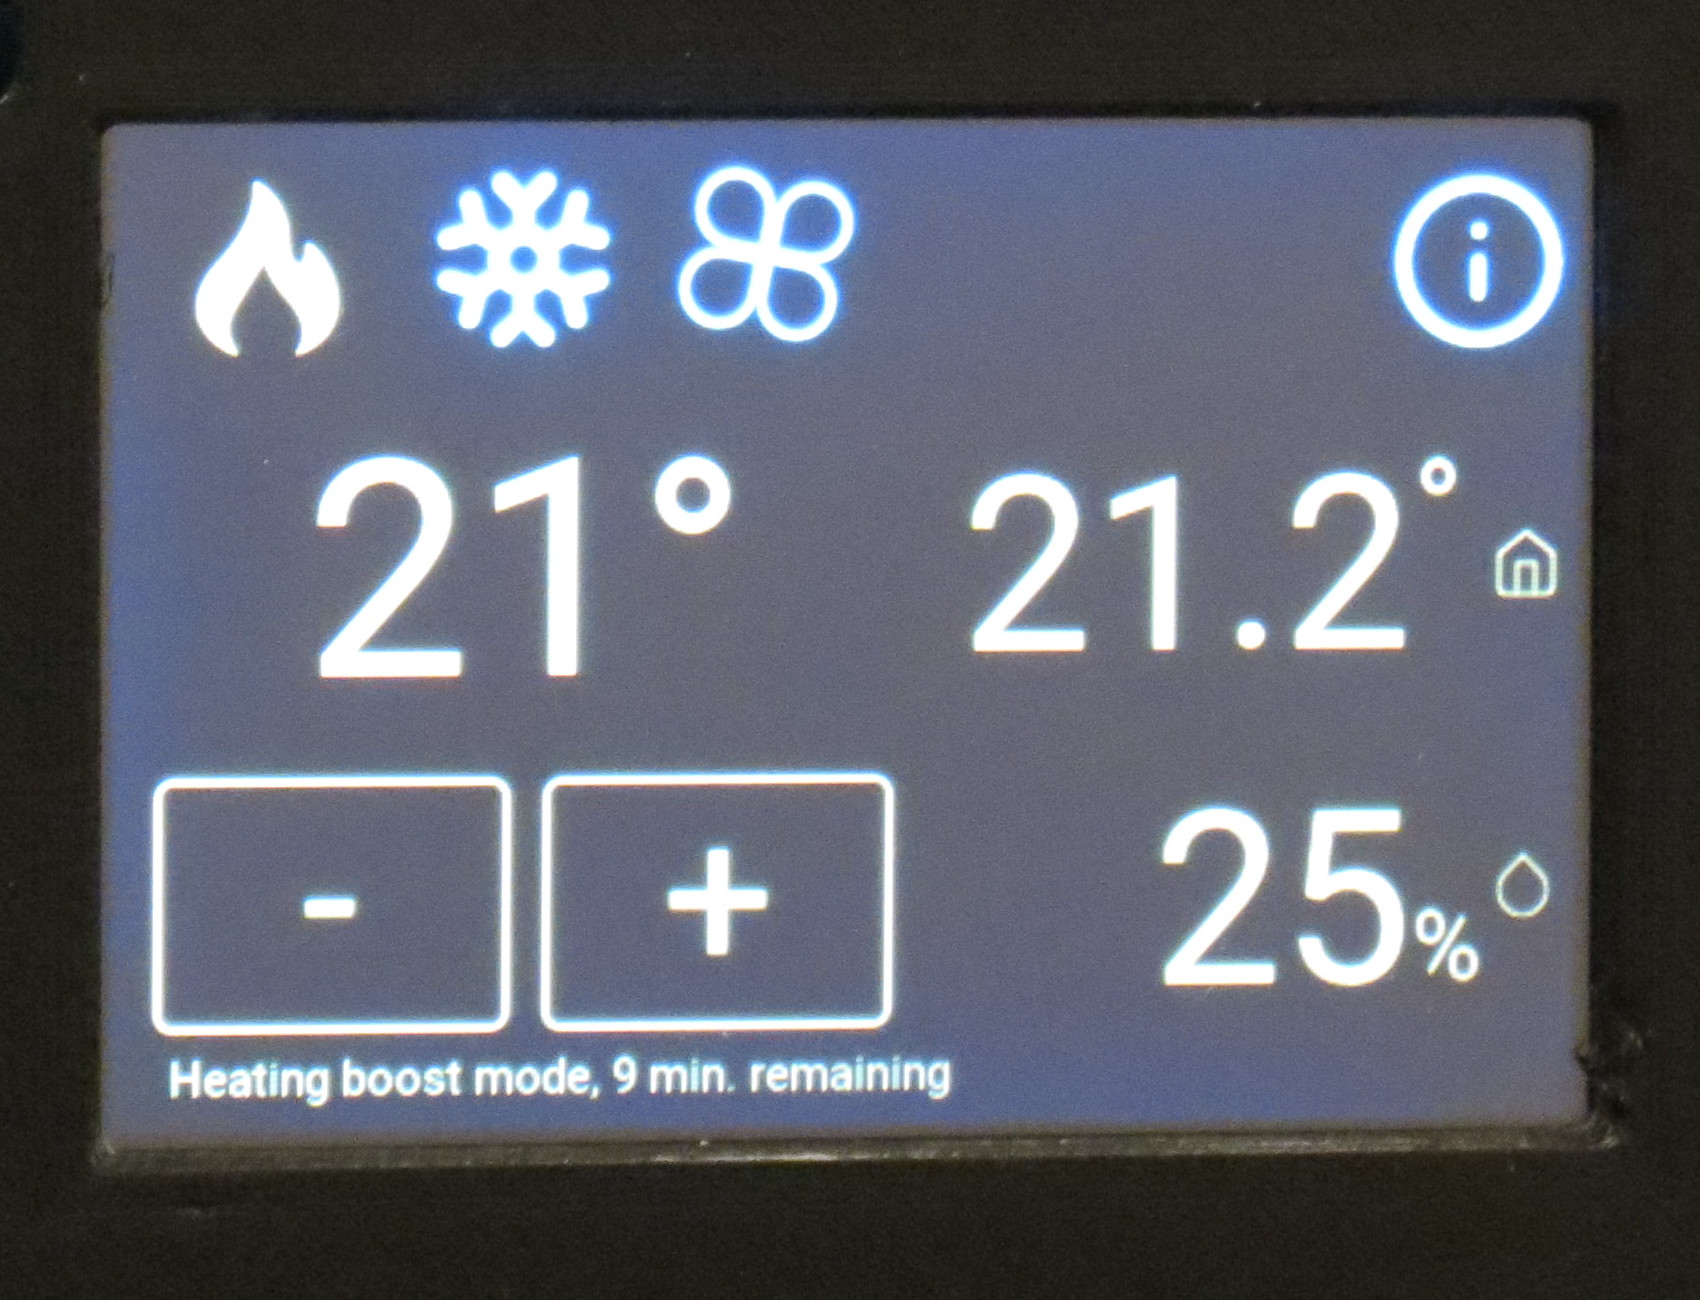
\includegraphics[width=.75\linewidth]{img/ui-heating-boost.jpg}
  \caption{Heating Interface - Boosting the heat}
  \label{fig:ui-heating-boost}
\end{subfigure}
\caption{fig:UI Menus}
\end{figure}

Pressing the flame icon in the upper left corner displays the heating menu.
In figure \ref{fig:ui-heating-off}, the status message at the bottom left
corner shows that the heating system is currently turned off.

Pressing the flame icon again, will activate the menu to turn on the heat
(see figure \ref{fig:ui-heating-menu}).  After turning on the heat, the set
temperature (displayed on the left) and the + and - buttons to change the set
point of the temperature will turn orange.  Figure \ref{fig:ui-heating-on}
shows the interface after turning up the temperature to a reasonable point.

Finally, one of the menu options in the menu to turn on the heat is ``boost''.
This is used to turn on the heat for a specified duration (default is 10
minutes) even if the temperature is already above the set point.  When the
system is in boost mode, this will be indiacted along with the duration of the
boost remaining in the bottom left corner of the heating menu, as showin in
figure \ref{fig:ui-heating-boost}.
